\section{Résultats}

\paragraph*{Pouvoir calorifique théorique du mélange éthanol-méthanol}
TODO: REVOIR CA STP, UTILISER LE TABLEAU\\
Conformément aux \autoref{eq:chaleur_réaction}, \autoref{eq:ethanol_combustion} et \autoref{eq:methanol_combustion} il est possible de calculer le pouvoir calorifique du mélange, c'est-à-dire la chaleur que sa combustion libère. Pour ce faire il est nécessaire de connaître sa chaleur de formation \(\Delta H_{l} = (-276 \pm 2)\) \si{\kilo\joule\per\mol} et sa masse molaire \(\rho_e = (46.1 \pm 0.1)\) \si{\gram\per\mol} \cite{ethanol-values}. Les valeurs des chaleurs de formation pour le \(CO_2\) et l'\(H_2O\) sont également nécessaires \cite{notice}. La valeur théorique obtenue pour le pouvoir calorifique de l'éthanol est donc \(H_{ethanol} = (26.8 \pm 0.1)\) \si{\mega\joule\per\kilo\gram}.







\paragraph*{Pouvoir calorifique théorique du butane-propane}
A l'aide des \autoref{eq:chaleur_réaction}, \autoref{eq:butane_combustion} et \autoref{eq:propane_combustion} il est possible de calculer le pouvoir calorifique du mélange butane-propane, c'est-à-dire la chaleur que sa combustion libère. Il s'agit d'abord de calculer le pouvoir calorifique de ses deux composants. Pour le butane, sa chaleur de formation est de \(\Delta H_{g} = (-125.6 \pm 0.7)\) \si{\kilo\joule\per\mol} et sa masse molaire est de \(\rho_b = (58.1 \pm 0.1)\) \si{\gram\per\mol} \cite{butane-values}. Pour le propane, celles-ci sont \(\Delta H_{g} = (-104.7 \pm 0.5)\) \si{\kilo\joule\per\mol} et \(\rho_p = (44.1 \pm 0.1)\) \si{\gram\per\mol} \cite{propane-values}. A l'aide des valeurs des chaleurs de formation du \ce{CO2} et de l'\ce{H2O} \cite{notice} il est possible d'obtenir le pouvoir calorifique du butane \(H_{butane} = (45.7 \pm 0.1)\) \si{\mega\joule\per\kilo\gram} et celui du propane \(H_{propane} = (46.3 \pm 0.1)\) \si{\mega\joule\per\kilo\gram}.

Afin d'obtenir le pouvoir calorifique théorique du mélange butane-propane il est nécessaire de connaître les proportions de chaque composant. Dans le mélange utilisé le butane composait 80\% du mélange et le propane 20\%. La supposition a été faite que le pouvoir calorifique du mélange correspondait à la moyenne pondérée par leur proportion de ces deux composants. La valeur obtenue est donc de \(H_{melange} = (45.8 \pm 0.1)\) \si{\mega\joule\per\kilo\gram}.





\paragraph*{Analyse expérimentale de la combustion de l'éthanol}
Les valeurs du pouvoir calorifique de la combustion de l'éthanol sont calculées avec l'\autoref{eq:pouvoir_calorifique}. À la fin de toutes les mesures, une masse d'eau de condensation totale \(\Delta M_\textrm{c,tot} = (4.8 \pm 0.1)\) \si{\gram} a été récupérée, donnant une masse \(\Delta M_c = (0.30 \pm 0.01)\) \si{\gram}. La mesure a été effectuée 16 fois et les résultats sont reportés dans la \autoref{fig:H_etanol}. La formule pour le calcul des erreurs est donné dans l'\autoref{sec:erreurs}. La valeur moyenne \(\langle H \rangle\) des mesures est reportée dans le \autoref{tab:pouvoir_calorifique}.

\paragraph*{Analyse expérimentale de la combustion du butane-propane}
En suivant le même procédé, le pouvoir calorifique de la combustion du mélange butane-propane a été déterminée. La masse d'eau condensée totale était \(\Delta M_\textrm{c,tot} = (37.6 \pm 0.1)\) \si{\gram}, donnant alors \(\Delta M_c = (3.13 \pm 0.01)\) \si{\gram} sur chaque mesure. Les résultats des 12 mesures effectuées sont visibles dans la \autoref{fig:H_gaz_camping}. La valeur moyenne \(\langle H \rangle\) des mesures est reportée dans le \autoref{tab:pouvoir_calorifique}.

L'écart relatif entre les valeurs théoriques \(H_\textrm{théo}\) et expérimentales \(H_\textrm{exp}\) sont calculés avec l'\autoref{eq:ecart_rel}

\begin{figure}[h]
    \centering
    \begin{subfigure}{0.5\linewidth}
        \centering
        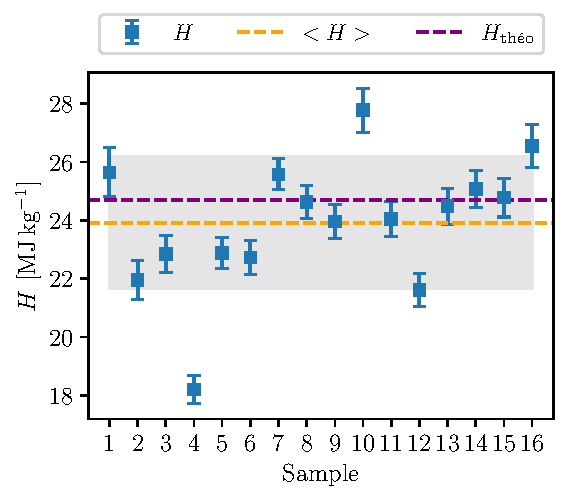
\includegraphics[width=\linewidth]{figures/ethanol.pdf}
        \caption{}
        \label{fig:H_etanol}
    \end{subfigure}%
    \begin{subfigure}{0.5\linewidth}
        \centering
        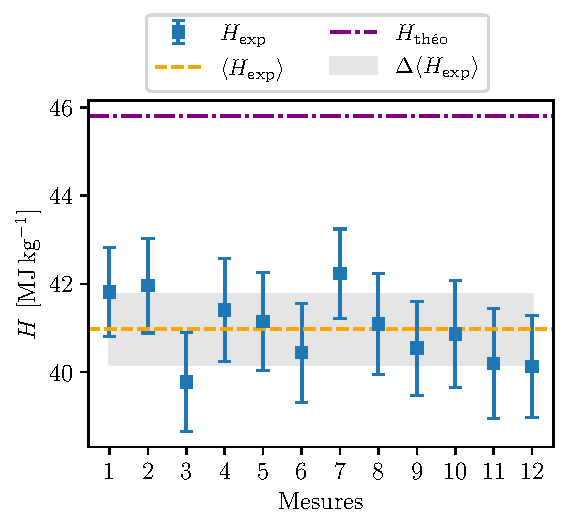
\includegraphics[width=\linewidth]{figures/gaz_camping.pdf}
        \caption{}
        \label{fig:H_gaz_camping}
    \end{subfigure}
    \caption{Pouvoirs calorifiques de combustion calculés pour (a) l'éthanol (b) le gaz de camping (80\% Butane, 20\% Propane)}
\end{figure}

\begin{table}[h]
    \centering
    \begin{tabulary}{\linewidth}{C C C C}
        \toprule
        Combustible & \(H_\textrm{théo}\) [\si{\mega\joule\per\kilo\gram}] & \(\langle H_\textrm{exp} \rangle\) [\si{\mega\joule\per\kilo\gram}] & Écart relatif \(a\) \\
        \midrule
        88\% Éthanol 12\% Méthanol & \(26.8 \pm 0.1\) & \(24 \pm 2\) & \(10.6 \pm 0.7\)\%\\
        80\% Butane 20\% Propane & \(45.8 \pm 0.1\) & \(41 \pm 1\) & \(10.7 \pm 0.6\)\% \\
        \bottomrule
    \end{tabulary}
    \caption{Valeurs théoriques et expérimentales des combustibles}
    \label{tab:pouvoir_calorifique}
\end{table}

\paragraph*{\ce{CO2} produit}
Le \ce{CO2} produit lors de la combustion est donné par l'\autoref{eq:masse_co2}. Puisque le débit était constant, deux mesures avec une masse d'eau \(\Delta M\) donnent un temps de combustion similaire. La quantité de \ce{CO2} produit 
